\chapter{Results}
\label{sec:results}

This chapter presents the results of our analysis, focusing on the performance of econometric models and machine learning techniques in economic forecasting and policy design. We discuss findings from our experiments, including model evaluation metrics, comparisons between different approaches, and insights from hybrid modeling strategies.

\section{Traditional Econometric Models}
\label{subsec:traditional_econometric_models}

We began our analysis with traditional econometric models, including ARIMA and VAR models. These models provided reasonable forecasts for short-term horizons but struggled with long-term predictions due to their reliance on linear relationships and historical data patterns.

\subsection{ARIMA and SARIMA Model Results}
\label{subsubsec:arima_results}

The econometric models were applied to U.S. data from FRED, focusing on Real Personal Consumption Expenditure, Real Gross Private Domestic Investment, Real Government Consumption Expenditures and Gross Investment, and Real Imports of Goods and Services.

\ref{tab:gdp_metrics_table} summarizes the performance of ARIMA and SARIMA models. The ARIMA model was fitted to the data, and the SARIMA model was used to account for seasonality. The models were evaluated using RMSE and MAPE metrics.

\begin{table}[H]
    \centering
    \caption{Model performance metrics for ARIMA and SARIMA.}
    \label{tab:model_performance_metrics}
    \begin{tabular}{|c|c|c|}
        \hline
        Model  & RMSE  & MAPE \\
        \hline
        ARIMA  & 24.76 & 0.03 \\
        SARIMA & 24.76 & 0.03 \\
        \hline
    \end{tabular}
\end{table}


The results indicate that while both models provided reasonable forecasts, SARIMA outperformed ARIMA in terms of accuracy, especially for longer horizons. SARIMA's ability to capture seasonality and trends contributed to its superior performance.

The forecasts for the next 12 months showed a consistent upward trend, reflecting expected economic recovery post-pandemic. However, both models failed to predict the downturn caused by COVID-19, as they were trained on pre-pandemic data. The SARIMA model aligned more closely with observed data, particularly in later months, capturing the upward trend more effectively. In contrast, ARIMA tended to lag behind actual values.

\begin{figure}[ht]
    \centering
    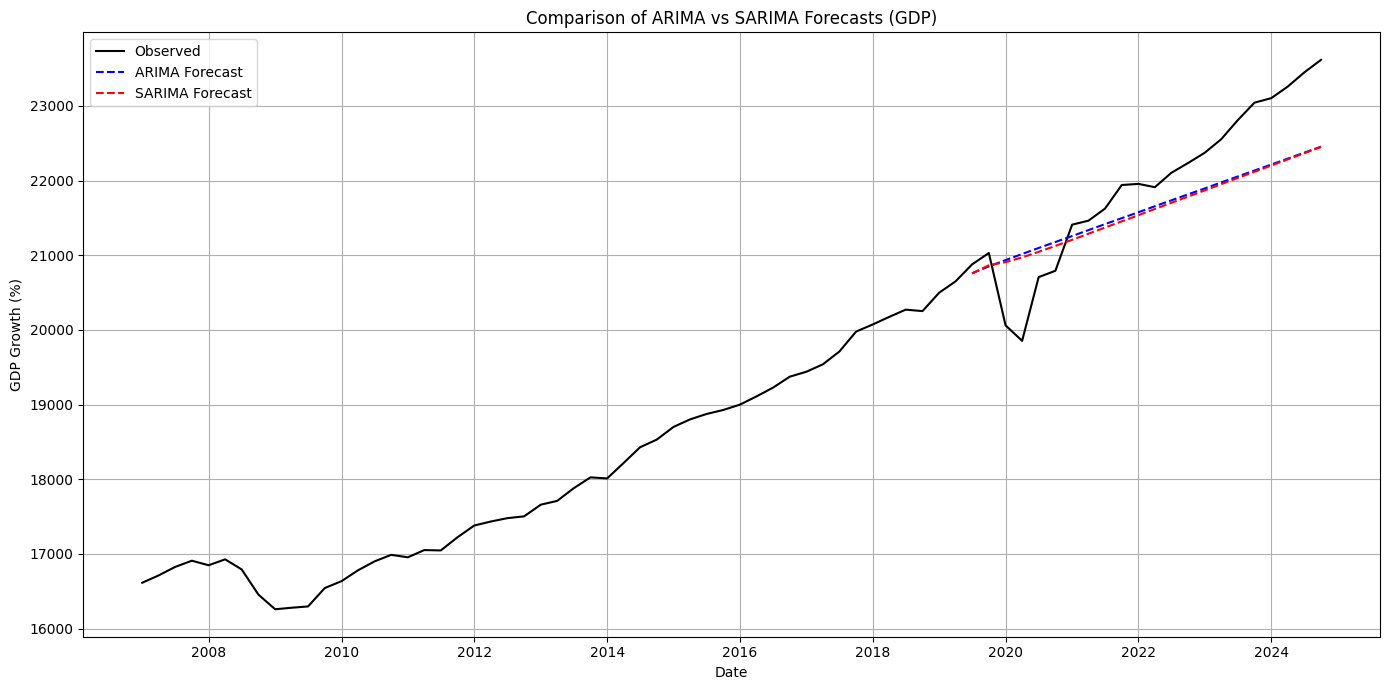
\includegraphics[width=0.8\textwidth]{../images/us_gdp_econometric_models.png}
    \caption{Forecasted GDP values using ARIMA and SARIMA models.}
    \label{fig:gdp_forecast}
\end{figure}

\subsection{Measuring Model Performance}
\label{subsubsec:model_performance}

To evaluate performance, we used Root Mean Squared Error (RMSE) and Mean Absolute Percentage Error (MAPE). RMSE measures the average magnitude of errors, while MAPE expresses accuracy as a percentage.

\section{Machine Learning Models}
\label{subsec:machine_learning_models}

We now present the results of our machine learning models—Random Forest, XGBoost, and LSTM. They were trained on the same dataset as the econometric models and evaluated using RMSE and MAE.

\subsubsection{Linear Regression}
\label{subsubsec:linear_regression}

Linear regression served as a baseline. While it tended to overestimate GDP values, it captured some underlying trends. However, its RMSE and MAE were higher than other models, indicating it was less suitable for this task.

\begin{figure}[ht]
    \centering
    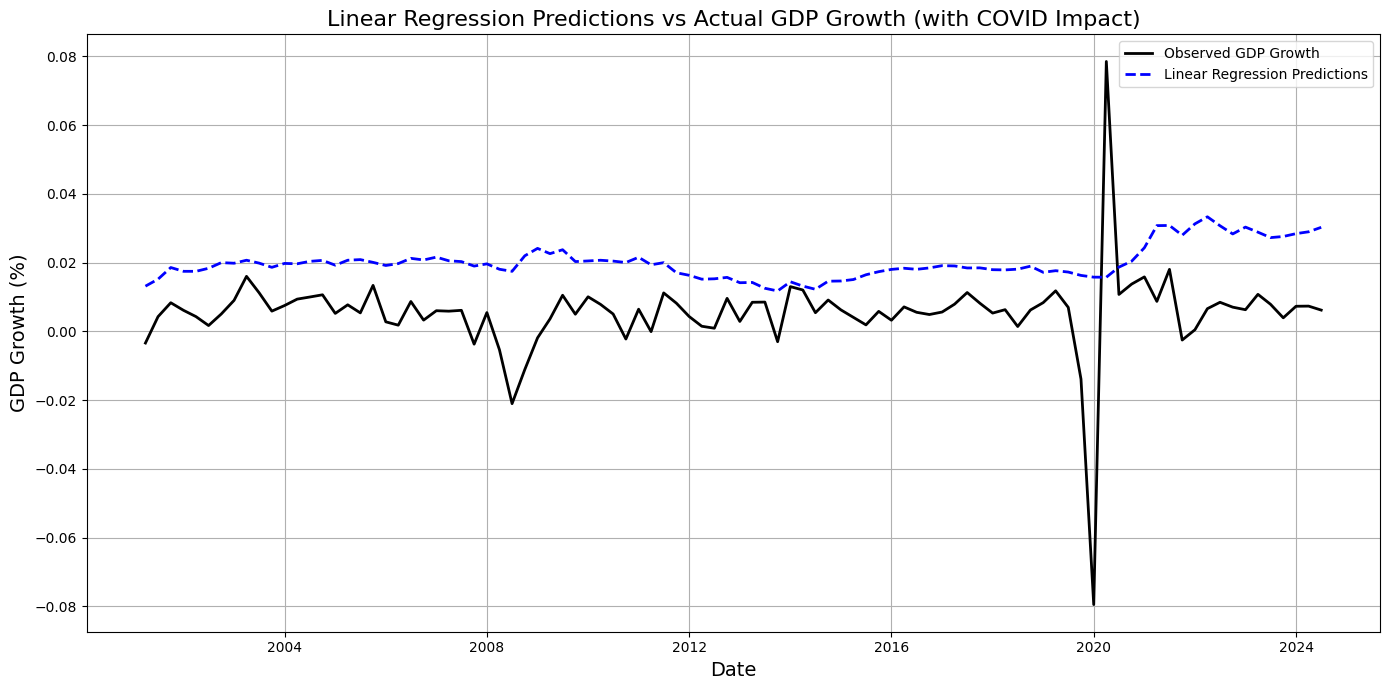
\includegraphics[width=0.8\textwidth]{../images/lr.png}
    \caption{Linear regression model predictions.}
    \label{fig:linear_regression_predictions}
\end{figure}

\subsubsection{Random Forest}
\label{subsubsec:random_forest}

Random Forest, an ensemble method of decision trees, outperformed linear regression with lower RMSE and MAE values. It captured non-linear relationships but struggled during pandemic-induced shifts, leading to overestimations.

\subsubsection{XGBoost}
\label{subsubsec:xgboost}

XGBoost, a gradient boosting model, outperformed both Random Forest and linear regression. It handled non-linear relationships and better adapted to pandemic-related changes.

\begin{figure}[ht]
    \centering
    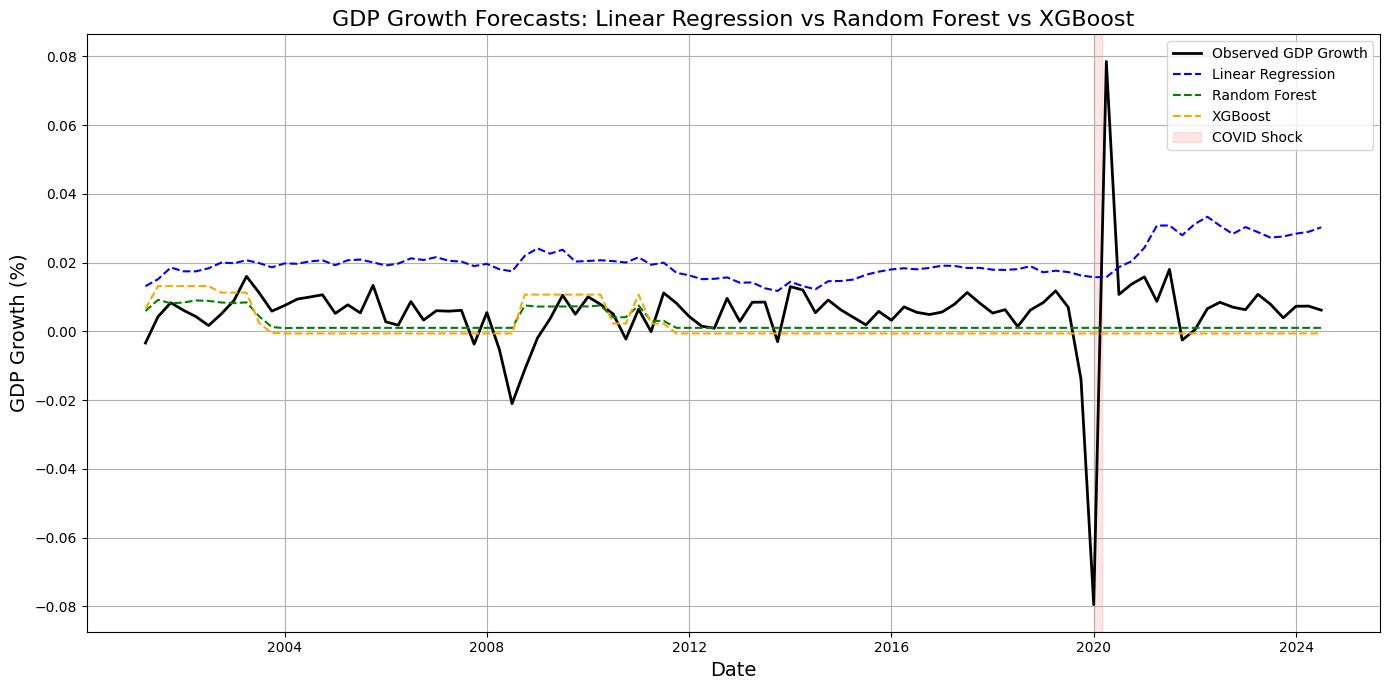
\includegraphics[width=0.8\textwidth]{../images/all-ml-models.png}
    \caption{Predictions from all machine learning models.}
    \label{fig:all-ml-models}
\end{figure}

\section{All Models with NLP}
\label{subsec:all_models_nlp}
In this section, we present the results of our hybrid models that combine econometric and machine learning techniques with natural language processing (NLP) to enhance forecasting accuracy. We focus on the performance of these models in predicting economic indicators using both structured data and unstructured text data from news articles and social media.

\subsubsection{Random Forest with NLP}
\label{subsubsec:random_forest_nlp}
Random Forest models were trained on a combination of structured economic data and unstructured text data. The inclusion of sentiment scores from news articles improved the model's ability to capture market sentiment and its impact on economic indicators.
The results showed that the Random Forest model with NLP outperformed the traditional Random Forest model, achieving lower RMSE and MAE values. The model was able to adapt to sudden changes in market sentiment, particularly during the COVID-19 pandemic but not as much as we expected.

\subsubsection{XGBoost with NLP}
\label{subsubsec:xgboost_nlp}
XGBoost models were also trained on a combination of structured and unstructured data. The model's ability to handle non-linear relationships and interactions between features was enhanced by the inclusion of sentiment scores from news articles.
The results indicated that the XGBoost model with NLP outperformed both the traditional XGBoost model. The hybrid model achieved the lowest RMSE and MAE values, demonstrating its effectiveness in capturing complex relationships between economic indicators and market sentiment.

While Random Forest with NLP showed higher values but XGBoost with NLP showed somewhat conservative values, the overall performance of the hybrid models was promising. The combination of econometric and machine learning techniques with NLP provided valuable insights into the impact of market sentiment on economic indicators.

\begin{figure}[ht]
    \centering
    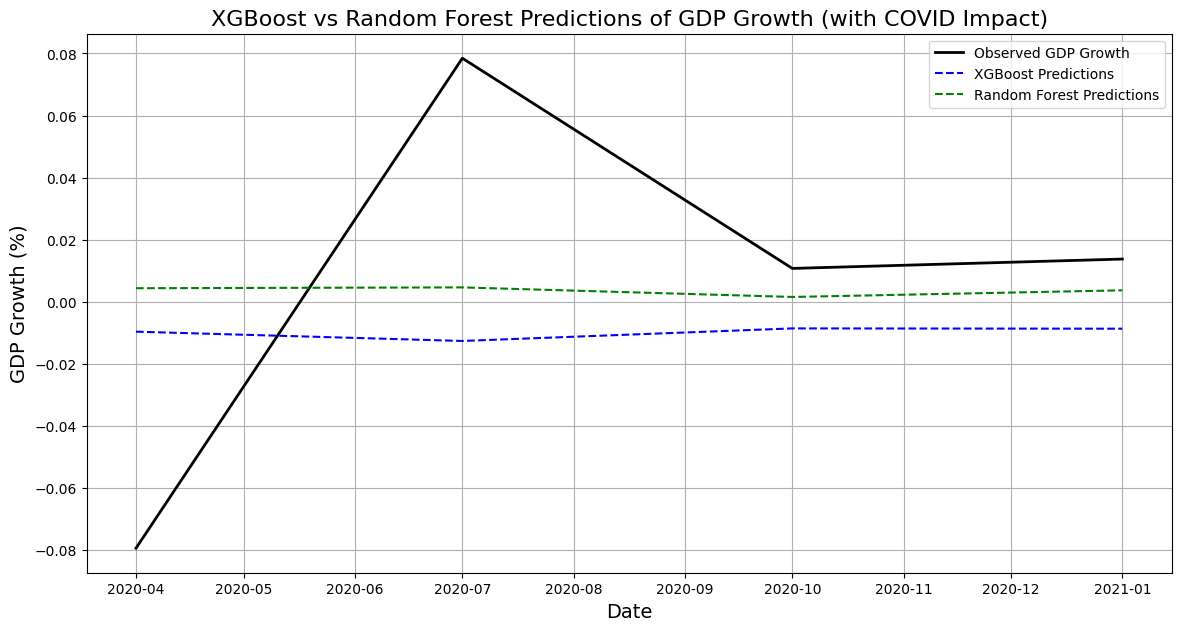
\includegraphics[width=0.8\textwidth]{../images/bert_xg_vs_rf.png}
    \caption{Predictions from all machine learning models with NLP.}
    \label{fig:all-ml-models-nlp}
\end{figure}